%%%%%%%%%%%%%%%%%%%%%%%%%%%%%%%%%%%%%%%%%%%%%%%%%%%%%%%%%%%%%%%%%%%%%%
%
%         Copyright (c) 2023, gitlabci_gallery / latex
%         All rights reserved.
%
%%%%%%%%%%%%%%%%%%%%%%%%%%%%%%%%%%%%%%%%%%%%%%%%%%%%%%%%%%%%%%%%%%%%%%

\documentclass[A4,svgnames,9pt,aspectratio=169]{beamer}
%% document options:
%% - aspectratio = { 43, 169, 1610 }
%% - utf8
%%


\setlength{\footskip}{300pt}
\usepackage[french]{babel}

\hypersetup{
   allcolors   = rouge_inria,
   pdfauthor   = {Duzés Florian},
   pdftitle    = {\@title},
   pdfsubject  = {Point hebdomadaire, bi-mensuel du stage},
   pdfkeywords = {entretien, observation du travail}
}

%%%%%%%%%%%%%%%%%%%%%%%%%%%%%%%%%%%%%%%%%%%%%%%%%%%%%%%
%%
%%%%%%%%%%%%%%%%%%%%%%%%%%%%%%%%%%%%%%%%%%%%%%%%%%%%%%%

\title[titrecourt]{Réunion flash}
\subtitle{Point hebdomadaire}
\date[23/07/2025]{date long}
\author[Duzes Florian]{Duzés Florian}

\usetheme{inria}


\begin{document}

%%%%%%%%%%%%%%%%%%%%%%%%%%%%%%%%%%%%%%%%%%%%%%%%%%%%%%%
%%
%%%%%%%%%%%%%%%%%%%%%%%%%%%%%%%%%%%%%%%%%%%%%%%%%%%%%%%

\frame{\titlepage}

%%%%%%%%%%%%%%%%%%%%%%%%%%%%%%%%%%%%%%%%%%%%%%%%%%%%%%%

% Le titre des planches de sommaire est \contentsname, sa valeur
% est fixée ici à "Sommaire" par défaut.
\renewcommand{\contentsname}{Sommaire}

\frame{\tocpage}


%%--%%--%%--%%--%%--%%--%%--%%--%%--%%--%%--%%--%%--%%--%%
 
\section{État des lieux}
\frame{\sectionpage}

\begin{frame}{Point actuel}
  \begin{tikzpicture}[
    node distance=2cm,
    box/.style={rectangle, draw=black, thick, minimum width=3cm, minimum height=1cm, text centered, rounded corners, font=\bfseries},
    arrow/.style={->, >=Stealth, thick, draw=arrowColor},
    contentBoxDone/.style={rectangle, draw=black, thick, fill=board_lightGray!40, rounded corners, minimum width=3cm, minimum height=2cm, text width=3cm, align=center},
    contentBox/.style={rectangle, draw=black, thick, rounded corners, minimum width=3cm, minimum height=2cm, text width=3cm, align=center}
]

    % DESSINS
    \node[box, fill=faitColor] (fait) {Fait};
    \node[box, fill=enCoursColor, right=of fait] (en_cours) {En cours};
    \node[box, fill=aFaireColor, right=of en_cours] (a_faire) {Prévus};
    \draw[arrow] (fait) -- (en_cours);
    \draw[arrow] (en_cours) -- (a_faire);

    % Choses réalisées
    % Choses réalisées
    \node[contentBoxDone, below=0.5cm of fait] {
      \begin{itemize}
        \item Remplir les config
        \item Appel des fonctions voisines
      \end{itemize}
      };
      
      % En cours
      \node[contentBox, below=0.5cm of en_cours, fill=enCoursColor!15] {
        \begin{itemize}
          \item Affiner la génération des tests pour \textit{Krmllib.h} et \textit{Hacl\_Hash\_Blake2b.h}
          \item Chaîne de bout en bout x86\_64 
          \item \textit{Introduction} du mémoire + section 1
        \end{itemize}
    };

    % Point fixer
    \node[contentBox, below=0.5cm of a_faire, fill=aFaireColor!15] {
        \begin{itemize}
            \item Couverture des architectures différentes
            \item Couverture des compilateurs
        \end{itemize}
    };
      \end{tikzpicture}


\end{frame}

%  .  .  .  .  .  .  .  .  .  .  .  .  .  .  .  .  .  .  %

\begin{frame}{Réalisation}
  \begin{tikzpicture}[
    node distance=2cm,
    box/.style={rectangle, draw=black, thick, minimum width=3cm, minimum height=1cm, text centered, rounded corners, font=\bfseries},
    arrow/.style={->, >=Stealth, thick, draw=arrowColor},
    contentBoxDone/.style={rectangle, draw=black, thick, fill=board_lightGray!40, rounded corners, minimum width=3cm, minimum height=2cm, text width=3cm, align=center},
    contentBox/.style={rectangle, draw=black, thick, rounded corners, minimum width=3cm, minimum height=2cm, text width=3cm, align=center}
]

    % DESSINS
    \node[box, fill=faitColor] (fait) {Fait};
    \node[box, fill=enCoursColor, right=of fait] (en_cours) {En cours};
    \node[box, fill=aFaireColor, right=of en_cours] (a_faire) {Prévus};
    \draw[arrow] (fait) -- (en_cours);
    \draw[arrow] (en_cours) -- (a_faire);

    % Choses réalisées
    \node[contentBoxDone, below=0.5cm of fait] {
      \begin{itemize}
        \item Remplir les config
        \item Appel des fonctions voisines
        \item Affiner la génération des tests pour \textit{Krmllib.h} et \textit{Hacl\_Hash\_Blake2b.h}
        \item Chaîne de bout en bout x86\_64 
      \end{itemize}
      };
      
      % En cours
      \node[contentBox, below=0.5cm of en_cours, fill=enCoursColor!15] {
        \begin{itemize}
          \item étude de résultat  
          \item Couverture des architectures différentes
          \item Couverture des compilateurs
        \end{itemize}
    };

    % Point fixer
    \node[contentBox, below=0.5cm of a_faire, fill=aFaireColor!15] {
        \begin{itemize}
          \item Mémoire de stage
        \end{itemize}
    };
      \end{tikzpicture}

\end{frame}

%%--%%--%%--%%--%%--%%--%%--%%--%%--%%--%%--%%--%%--%%--%%

\section{Axes de travails}
\frame{\sectionpage}

\begin{frame}{Organisation des modules}
  \centering
  \begin{tikzpicture}[auto]

    % Styles
    \tikzstyle{startstop} = [rectangle, rounded corners, minimum width=2cm, minimum height=1cm, text centered, draw=black, fill=green!30]
    \tikzstyle{process} = [rectangle, minimum width=2cm, minimum height=1cm, text centered, draw=black, fill=orange!30]
    \tikzstyle{arrow} = [thick,->,>=stealth]
    \tikzset{zone1/.style={rectangle, rounded corners, draw=red, dashed, fill=red!10, inner sep=0.3cm}}
    \tikzset{zone2/.style={rectangle, rounded corners, draw=blue, dashed, fill=blue!10, inner sep=0.3cm}}
    \tikzset{zone22/.style={rectangle, rounded corners, draw=none, fill=blue!10, inner sep=0.3cm}}
    \tikzset{zone3/.style={rectangle, rounded corners, draw=green, dashed, fill=green!10, inner sep=0.3cm}}
    
    % Noeuds
    \node (hacl) [startstop] {Hacl*};
    \node (c) [below of=hacl] {.h};
    \node (ini) [below of=c, xshift=2cm] {.ini};
    \node (test) [below of=c, xshift=-2cm] {-test.c};
    \node (script) [below of=c] {.script};
    \node (compilateur) [process, below of=test] {Compilateur};
    \node (exe) [below of=compilateur] {-test.exe};
    \node (blanc1) [below of=script] {};
    \node (blanc2) [below of=blanc1] {};
    \node (gdb) [process, below of=blanc2] {GDB};
    \node (snap) [right of=gdb, xshift=2cm] {.snapshot};
    \node (binsec) [startstop, right of=snap, xshift=1.5cm] {Binsec};
    
    % Flèches
    \draw [arrow] (hacl) -- (c);
    \draw [arrow] (c) -- (ini);
    \draw [arrow] (c) -- (test);
    \draw [arrow] (c) -- (script);
    \draw [arrow] (test) -- (compilateur);
    \draw [arrow] (compilateur) -- (exe);
    \draw [arrow] (exe) -- (gdb);
    \draw [arrow] (script) -- (gdb);
    \draw [arrow] (gdb) -- (snap);
    \draw [arrow] (snap) -- (binsec);
    \draw [arrow] (ini) -- (binsec);

    % Zones
    \begin{scope}[on background layer]
        \node [zone1, fit=(c) (ini) (test) (script)] {};
        \node [zone2, fit=(script) (gdb)] {};
        \node [zone2, fit=(gdb) (snap) (binsec)] {};
        \draw [zone22]
        ([xshift=-9pt, yshift=10pt]gdb.north west) --
        ([xshift=9pt, yshift=10pt]gdb.north east) -- 
        ([xshift=1pt, yshift=-1pt]gdb.south east) -- 
        ([xshift=-1pt, yshift=-1pt]gdb.south west) --
        cycle;
        \node [zone3, fit=(compilateur) (exe)] {};
    \end{scope}
    \end{tikzpicture}
\end{frame}

%  .  .  .  .  .  .  .  .  .  .  .  .  .  .  .  .  .  .  %

\begin{frame}{Division du travail}
  \centering
  \begin{tikzpicture}[auto]

    % Styles
    \tikzstyle{startstop} = [rectangle, rounded corners, minimum width=2cm, minimum height=1cm, text centered, draw=black, fill=green!30]
    \tikzstyle{process} = [rectangle, minimum width=2cm, minimum height=1cm, text centered, draw=black, fill=orange!30]
    \tikzstyle{arrow} = [thick,->,>=stealth]
    \tikzset{zone1/.style={rectangle, rounded corners, draw=red, dashed, fill=red!10, inner sep=0.3cm}}
    \tikzset{zone2/.style={rectangle, rounded corners, draw=blue, dashed, fill=blue!10, inner sep=0.5cm, text width=3cm}}
    \tikzset{zone3/.style={rectangle, rounded corners, draw=green, dashed, fill=green!10, inner sep=0.3cm}}
    \tikzset{zone4/.style={rectangle, rounded corners, draw=green, dashed, fill=green!30!blue!5, inner sep=0.3cm}}
    
    % Noeuds
    \node (make_test) [startstop] {ANDHRÍMNIR};
    \node (test) [below of = make_test] {make\_tests};
    \node (test1) [below of=test, xshift=0.5cm, yshift=0.6cm] {\small{test1}};
    \node (test2) [below of=test1, yshift=0.6cm] {\small{test2}};
    \node (test3) [below of=test2, yshift=0.6cm] {\small{test3}};
    \node (test4) [below of=test3, yshift=0.6cm] {\small{test4}};
    \node (dots) [below of=test4, yshift=0.6cm] {\small{$\dots$}};
    
    \foreach \node in {test1, test2, test3, test4, dots} {
      \draw (test.south) |- (\node.west);
      }
      
    \node (start) [startstop, right of=make_test, yshift=2cm, xshift = 4cm] {Érysichton};
    \node (blanc) [right of=make_test,yshift=-1cm, xshift = 2cm] {};
    \node (compilateur) [below of = start] {Compilateur};
    \node (hacl) [below of = compilateur, xshift=1cm] {\textit{\$}Hacl*};
    \node (tests) [below of = hacl, yshift = 0.3cm] {\textit{\$}tests};
    \node (binsec) [below of = tests, xshift=1cm] {\textit{\$}Binsec};
    \node (analyse) [below of = binsec, yshift = 0.3cm] {Analyse};
    % Flèches
    \draw [arrow] (compilateur.south) |- (hacl.west);
    \draw [arrow] (compilateur.south) |- (tests.west);
    \draw [arrow] (tests.south) |- (binsec.west);
    \draw [arrow] (tests.south) |- (analyse.west);

    % Zones
    \begin{scope}[on background layer]
        \node (zone2node) [zone2, fit=(start) (compilateur) (hacl) (tests) (binsec) (analyse) (make_test) (test) (test1) (test2) (test3) (test4) (dots)] {};
        \node (title) [anchor=north west] at (zone2node.north west) {\parbox{3cm}{\centering \Huge{\textbf{Érysichton}}\\\scriptsize{\textit{control panel}}}};
        \node (zone_tests) [zone1, fit=(make_test) (test) (test1) (test2) (test3) (test4) (dots)] {};
        \node (zone_compilation) [zone3, fit=(start) (compilateur) (hacl) (tests) (binsec) (analyse)] {};
        \node (zone_binsec) [zone4, fit=(binsec) (analyse)] {};
    \end{scope}

    % Flèches 2
    \onslide<2>{
    \draw [arrow, dashed, opacity=0.5] (title) -- (zone_tests);
    \draw [arrow, dashed, opacity=0.5] (title) -- (zone_compilation.west);
    \draw [thick,>=stealth, dashed, opacity=0.5] (title) -- (blanc.north);
    \draw [arrow, dashed, opacity=0.5] (blanc.north) -- (zone_binsec);
    \draw [arrow, dashed, opacity=0.2] (zone_tests.north) -- (zone_compilation.west);}
    \end{tikzpicture}
\end{frame}

% %%--%%--%%--%%--%%--%%--%%--%%--%%--%%--%%--%%--%%--%%--%%


\section{Andhrímnir}
\frame{\sectionpage}

\begin{frame}{Cuisinier immortel}
  
    \begin{block}{Ingrédients :}
      \begin{itemize}
        \item fichier .h
        \item fichier de config (particulier ou blanc)
      \end{itemize}
    \end{block}

    \begin{block}{Recette :}
      \begin{itemize}
        \item \textit{\$ make tests}
      \end{itemize}
    \end{block}

    \onslide<2>{On obtient \textbf{548} fichier C prêt à être compiler.}
\end{frame}

%  .  .  .  .  .  .  .  .  .  .  .  .  .  .  .  .  .  .  %

\begin{frame}{Points d'amélioration}

  \begin{block}{Limitations}
      \begin{itemize}
        \item dépendances aux fichier de config
        \item aucune ouverture à de nouveaux fichiers
      \end{itemize}
  \end{block}


\end{frame}

%%%%%%%%%%%%%%%%%%%%%%%%%%%%%%%%%%%%%%%%%%%%%%%%%%%%%%%

\section{Érysichton}
\frame{\sectionpage}

\begin{frame}{On aurait pu le nommer Sisyphe}
  
  \begin{block}{Module x86\_64 achevé}
    \centering
    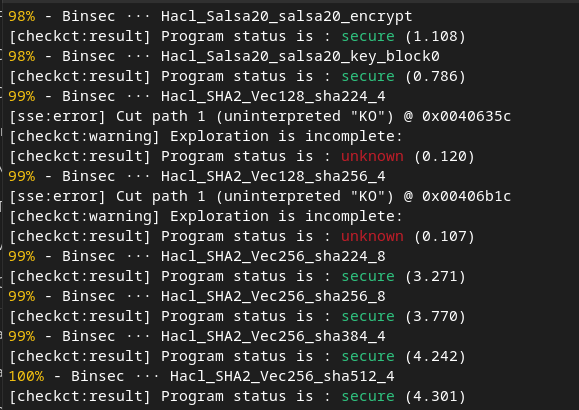
\includegraphics[scale = 0.4, trim= 6pt 0pt 0pt 0pt, clip]{imgs/Capture d’écran du 2025-07-23 11-01-55.png}
  \end{block}

\end{frame}

%  .  .  .  .  .  .  .  .  .  .  .  .  .  .  .  .  .  .  %

\begin{frame}{Statistiques - 1}
  \begin{table}[h]
    \centering
    \begin{tabular}{|c|c|c|c|}
      \hline
      & \textbf{Secure} & \textbf{Unknown} & \textbf{Insecure} \\
      \hline
      \textbf{Result} & 436 & 112 & 0 \\
      \hline
      \textbf{(\%)} & 79.37 & 20.43 & 0 \\
      \hline
    \end{tabular}
    \caption{Résultats pour une compilation sur x86\_64, \textit{gcc 12.2.0}}
    \label{tab:simple}
  \end{table}
\end{frame}

%  .  .  .  .  .  .  .  .  .  .  .  .  .  .  .  .  .  .  %

\begin{frame}{Statistiques - 2}
  \begin{table}[h]
    \centering
    \begin{tabular}{|c|c|c|c|}
      \hline
      \textbf{Unknown} &  & \\
      \hline
      \textit{Total} &  & 112 \\
      \hline
      \hline
      \textit{error} &  & 60 \\
      \hline
      -- & uninterpreted "syscall" & 21 \\
      \hline
      -- & uninterpreted "KO" & 39 \\
      \hline
      \textit{warning} & max depth & 52 \\
      \hline
    \end{tabular}
    \caption{Détails erreurs}
    \label{tab:unknown}
  \end{table}
\end{frame}

%  .  .  .  .  .  .  .  .  .  .  .  .  .  .  .  .  .  .  %


\begin{frame}[fragile]{Script Binsec}
  \begin{columns}
    \begin{column}{0.5\textwidth}
      \begin{lstlisting}[style=INIStyle, caption={HFStar\_UInt64\_eq\_mask.ini}, gobble=8]
        starting from core
        halt at @[rsp, 8]
        explore all
      \end{lstlisting}
    \end{column}

    \begin{column}{0.5\textwidth}
      \begin{lstlisting}[style=INIStyle, caption={Hacl\_AEAD\_Chacha20Poly1305\_decrypt.ini}, gobble=8]
        starting from core
        secret global output, input, data, key, nonce, tag
        halt at @[rsp, 8]
        explore all
      \end{lstlisting}
    \end{column}
  \end{columns}
\end{frame}

%  .  .  .  .  .  .  .  .  .  .  .  .  .  .  .  .  .  .  %

\section*{Flash info}
\frame{\sectionpage}

\begin{frame}[fragile]{Script Binsec}

  \begin{lstlisting}[style=INIStyle, caption={\textbf{*}.ini}, gobble=4]
    starting from core
    halt at @[rsp, 8]
    explore all
  \end{lstlisting}



\end{frame}

%%%%%%%%%%%%%%%%%%%%%%%%%%%%%%%%%%%%%%%%%%%%%%%%%%%%%%%

\section{Conclusion}
\frame{\sectionpage}

\begin{frame}{Conclusion}
  \begin{block}{Objectif}
    \sout{Finir le module x86\_64.}
  \end{block}

  \begin{block}{Un oeil plus fin}
    Comprendre pourquoi ces erreurs -> affiner les scripts Binsec
  \end{block}
  
  \begin{block}{Augmenter}
    Ajouter d'autres compilateur
  \end{block}

\end{frame}

%%%%%%%%%%%%%%%%%%%%%%%%%%%%%%%%%%%%%%%%%%%%%%%%%%%%%%%

%% Le texte est modifiable en changeant \thankyou
%% \renewcommand{\thankyou}{Thank You.}
\frame{\merci}


\end{document}

